Neste capítulo apresenta-se os métodos experimentais utilizados para 
quantificação das concentrações de massa total, das espécies químicas e 
do Black Carbon nas amostras. Empregou-se, respectivamente:
Análise gravimétrica, Fluorescência de raios X (XRF),
Thermal/Optical Transmittance (TOT) e Refletância.
Apresenta-se sinteticamente o desenvolvimento teórico de cada método, bem como 
as condições de uso, procedimentos de calibração, cálculo das incertezas, 
vantagens e desvantagens, entre outros.

Para resolução dos modelos receptores, expõe-se também os métodos 
estatísticos Análise de Fatores e Positive Matrix Factorizarion (PMF) 
usados na identificação dos perfis de fontes. 

Desensolve-se ainda, uma metodologia para estimativa das incertezas
da calibração da XRF e Refletância, fundamentais para análises de PMF,
cuja metodologia emprega a ponderação pelas incertezas.

%%%%
\section{Amostragem}
% http://maps.google.com/maps/ms?ie=UTF8&hl=en&msa=0&msid=116003586198857296821.00046d7e7367b947abe12&z=12

\begin{figure}[H]
\begin{center}
  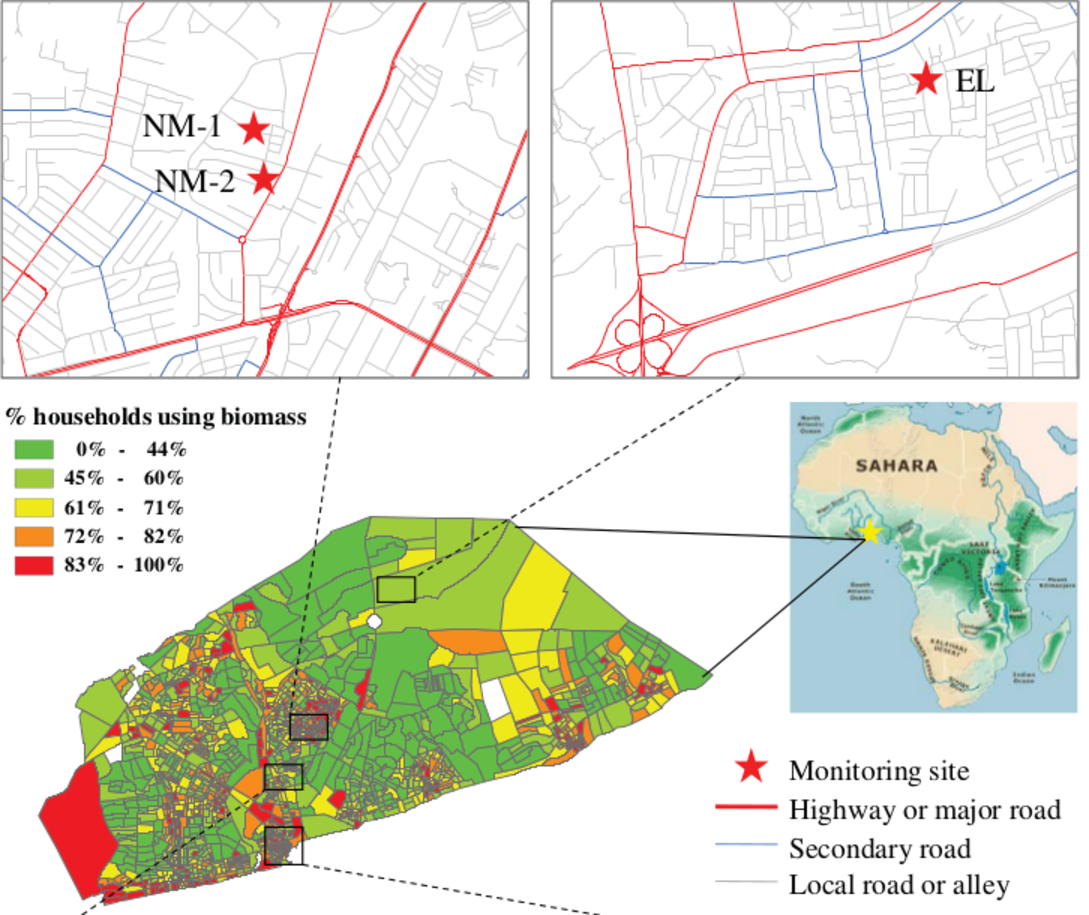
\includegraphics[width=0.6\textwidth]{../inputs/images/zheng/nima_mapa.pdf}
  \caption{Mapa de Nima. NM-1 ponto de amostragem na área residencial e 
           NM-2 ponto de amostragem na avenida. Porcentagem do uso da queima
           de biomassa para preparação de alimentos em residências usando dados
           do censo de \citeyearpar{ghanacensus2003}. Imagem reproduzida do 
           artigo \citet{zhou2013}. \label{fig:nima_mapa}}
\end{center}
\end{figure}

A localização geográfica dos dois pontos de medição, distantes entre si 330
metros, é apresentada na figura
\ref{fig:nima_mapa}, sendo NM-1 na rua \textit{Sam Road}, quarteirão residencial,
e NM-2 na \textit{Nima Road}, via arterial de 2,8 km na direção norte-sul, 
direciona o tráfego de pequenas vias locais para o centro, atravessando áreas de 
comércio variado. 
%distante 5 km do aeroporto de Acra

As medições ocorreram entre 11 de novembro de 2006 e 15 de agosto de 2008 com 
amostragem de 48 horas de duração, com total de 879 amostras coletadas. 
Falta de eletricidade, problemas com amostrador, 
filtros danificados ou contaminado na manipulação e ausência do 
operador durante as trocas foram as principais ocorrências registradas, 
totalizando menos que 10\% de dias sem medidas. 

As amostras foram coletadas em filtro de composição de politetrafluoretileno
(PTFE), comercialmente conhecidos por teflon, com diâmetro de 37 mm e 
poros de 0,2 $\mu m$. A área média de deposição, 7,32 ($\pm$ 0,44) $cm^2$, 
foi calculada medindo-se a mancha de deposição com um leitor de espectros 
(nônio de centésimos de mm), sobre 12 filtros amostrados.

Para coleta do MP utilizou-se amostradores Harvard, descritos por 
\citet{marple1987}. Neste equipamento a seleção do diâmetro das partículas 
admitidas no amostrador é feita por impactação inercial. 
Para coleta de $MP_{10}$ o $D_{50}$ do sistema era de $10 \mu m$, 
com fluxo de 4,0 $L.min^{-1}$, enquanto que para $MP_{2,5}$ o $D_{50}$ 
era de $2,5 \mu m$, com fluxo de 5,0 $L.min^{-1}$, medido com 10\% de precisão. 

Filtros brancos de campo e de laboratórios foram separados para avaliar 
possíveis contaminações de fábrica ou de manipulação das amostras. 

Os filtros foram pesados no laboratório da HSPH, usando uma balança
microanalítica (Mettler Toledo MT5) com precisão de $\pm 1 \mu g$, 
em ambiente controlado [umidade ($39 \pm 2 \%$), 
temperatura ($20,5 \pm 0,2 ^{\circ} C$) e eliminação de cargas eletrostáticas 
com fonte de polônio]. Os filtros permaneciam ao menos 24 h na sala, 
antes da pesagem, calculando-se a média de duas pesagens que não diferissem 
por mais que $5 \mu g$.
